% Created 2017-09-07 Thu 11:03
\documentclass{article}
\usepackage[utf8]{inputenc}
\usepackage[T1]{fontenc}
\usepackage{fixltx2e}
\usepackage{graphicx}
\usepackage{longtable}
\usepackage{float}
\usepackage{wrapfig}
\usepackage{rotating}
\usepackage[normalem]{ulem}
\usepackage{amsmath}
\usepackage{textcomp}
\usepackage{marvosym}
\usepackage{wasysym}
\usepackage{amssymb}
\usepackage{hyperref}
\tolerance=1000
\usepackage{tabularx,graphicx,ragged2e,booktabs,caption,float}
\usepackage[margin=0.8in]{geometry}
\usepackage{amsmath}
\usepackage{gensymb}
\usepackage{authblk}
\setlength{\parskip}{0.2cm}
\setlength{\parindent}{0.85cm}
\author{Tiankai Xiong}
\date{\today}
\title{PC5215, Lab1}
\hypersetup{
  pdfkeywords={},
  pdfsubject={},
  pdfcreator={Emacs 25.2.1 (Org mode 8.2.10)}}
\begin{document}

\maketitle


\section{Question 1}
\label{sec-1}

\subsection{Elaboration}
\label{sec-1-1}

Instead of copying everything from \emph{Numerical Recipes},
\texttt{ludcmp} was rewritten with modifications such that it no
longer needs a \texttt{struct} to begin with. Simple functions such
as \texttt{double **initMat(int n)} are written to avoid repeated
work in creating square matrices.

In addition, to force \texttt{ludcmp} to decompose without pivoting, a
parameter \texttt{noPivot} is added so that when it is nonzero, \texttt{ludcmp} skip
the part where it swaps rows in the matrix.

The function \texttt{ludcmp} follows Crout's algorithm where the diagonal of
\texttt{L} is taken as 1 such that for an $N \times N$ matrix, we only have
$N^2 - N$ variables to be determined while $N^2$ equations are
available. The algorithm iterates from left to right, top to
bottom. The results are stored in the original matrix because
whenever a new value is determined on a certain site, the old value
will not be used anymore. The result matrix $A$ is such that the
lower triangle part(without the diagonal) are values for L while
the upper diagonal part with the diagonal are values for U.

After the LU decomposition is determined, we use \texttt{lubksb} to solve
the linear system $Ax = b$ with $b$ given. Since we have $A = LU$,
the problem can be separated into two steps i.e.

$$L U x = b$$
$$L (U x) = b$$
$$L y = b$$
$$U x = y$$

where we solve for $y$ first, then $x$. It is worth mentioning that
\texttt{noPivot} parameter is also added for \texttt{ludksb} otherwise it will take
the \texttt{indx} array which stores the row permutations and reverse the
work accordingly.

\subsection{Results}
\label{sec-1-2}

Result from executing the compiled source code of
\texttt{lab1\_1.c} is presented in Fig \ref{fig:result1-1} which is
verified in Matlab as shown in Fig \ref{fig:matlab1} and Fig
\ref{fig:matlab2}. The answer to Q1 up to 6 digits is:
$$x = -0.214439$$
$$y = -1.265114$$
$$z = -0.536490$$
$$w = -1.123851$$

\begin{figure}
  \centering
  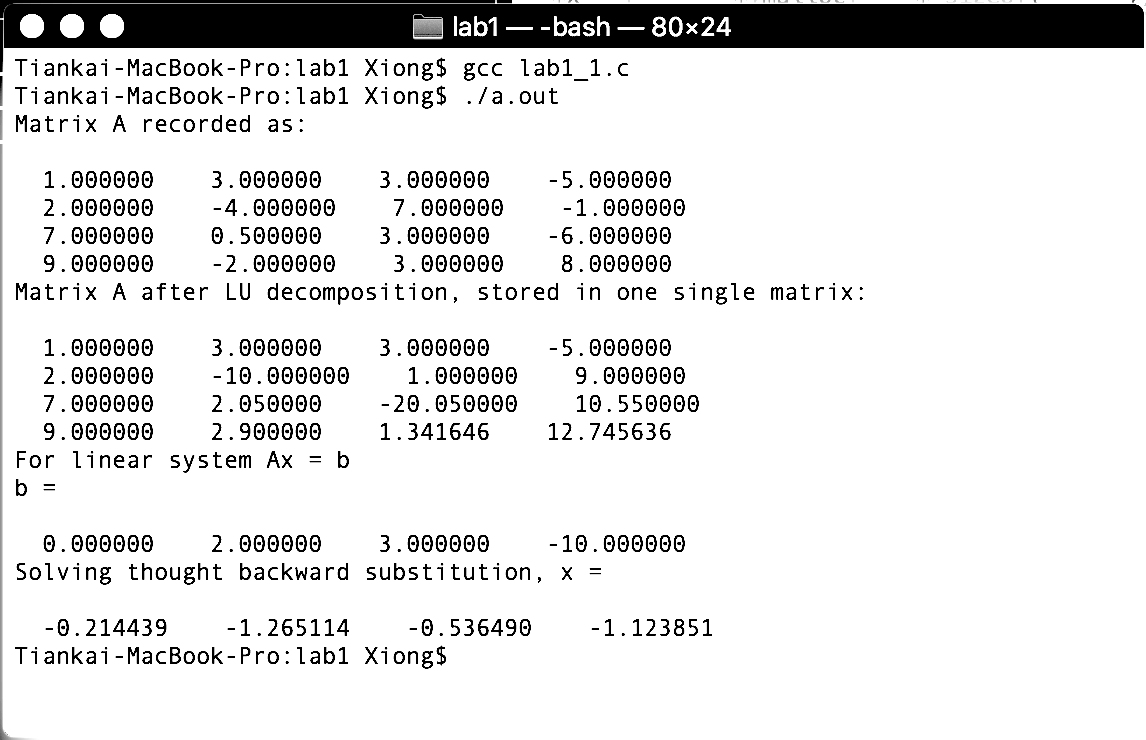
\includegraphics[width=0.6\textwidth]{result1-1.png}
  \caption{Result for Question 1}
  \label{fig:result1-1}
\end{figure}

\begin{figure}
  \centering
  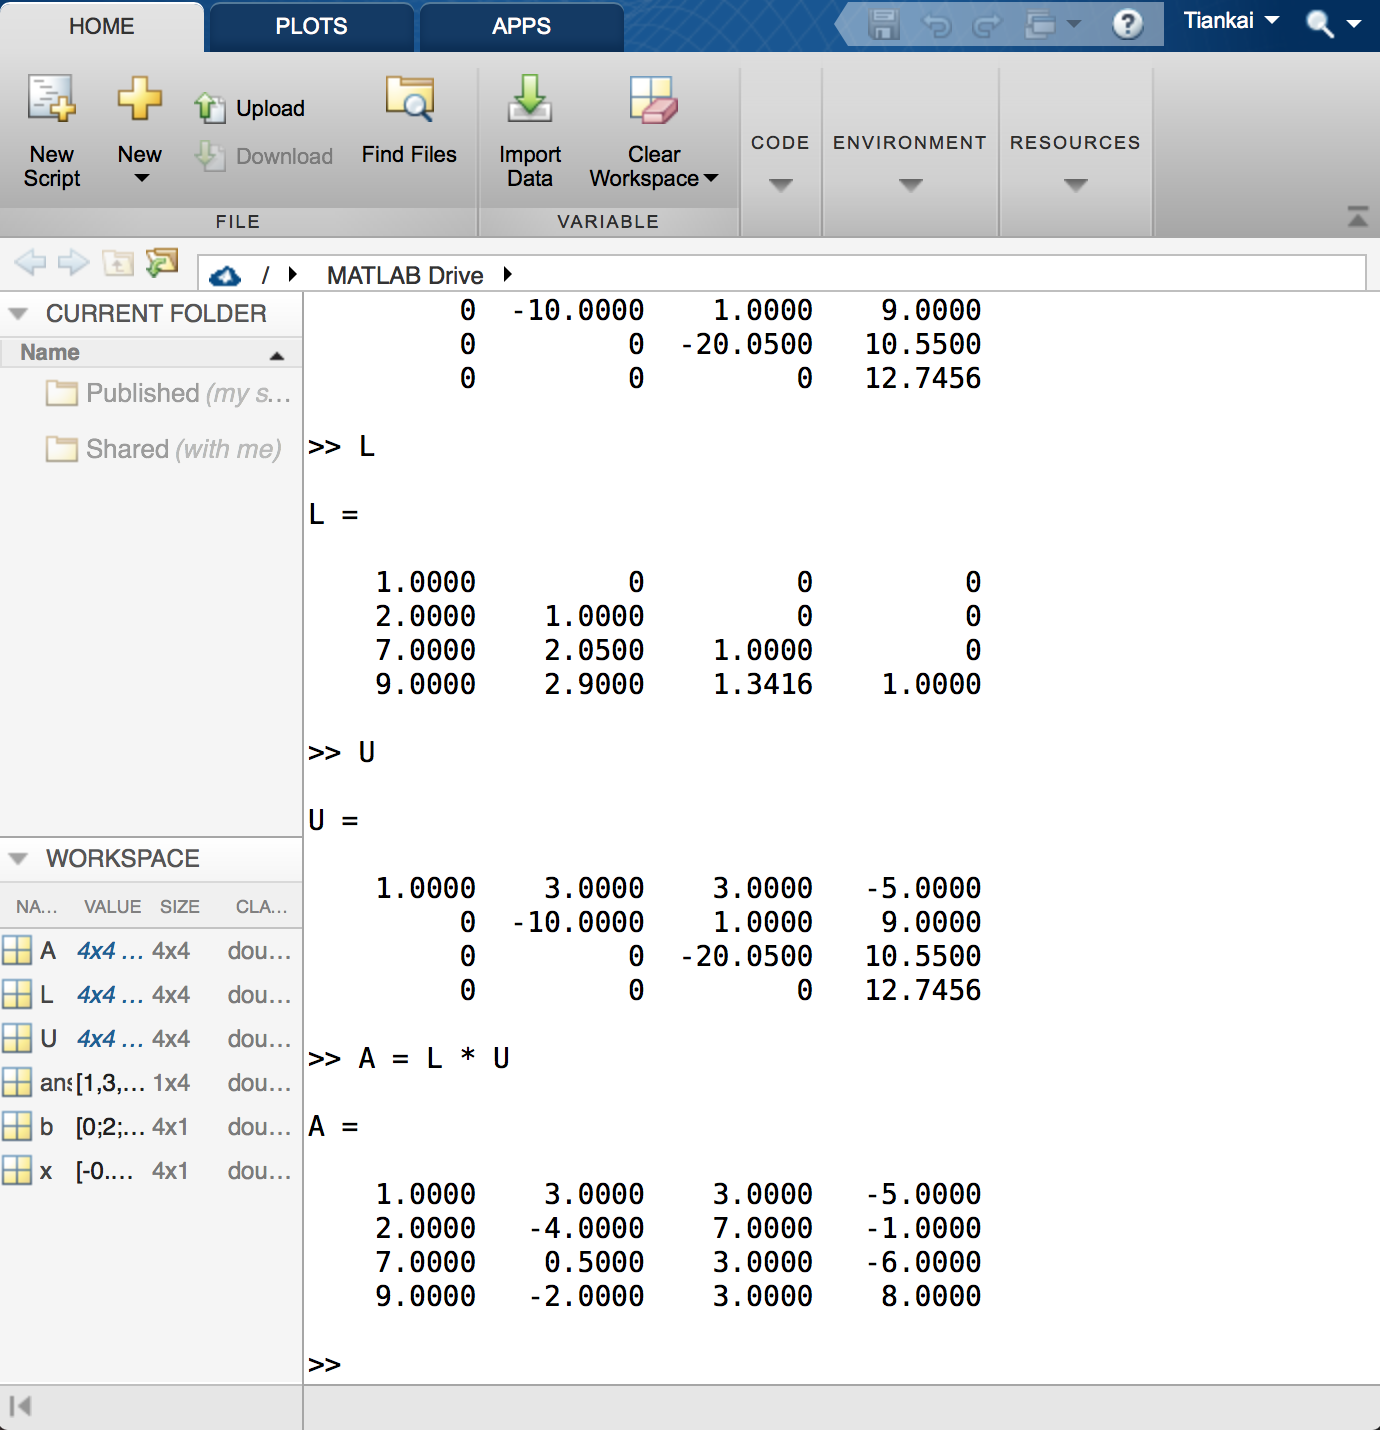
\includegraphics[width=0.6\textwidth]{matlab1.png}
  \caption{Verification of LU = A in Matlab}
  \label{fig:matlab1}
\end{figure}

\begin{figure}
  \centering
  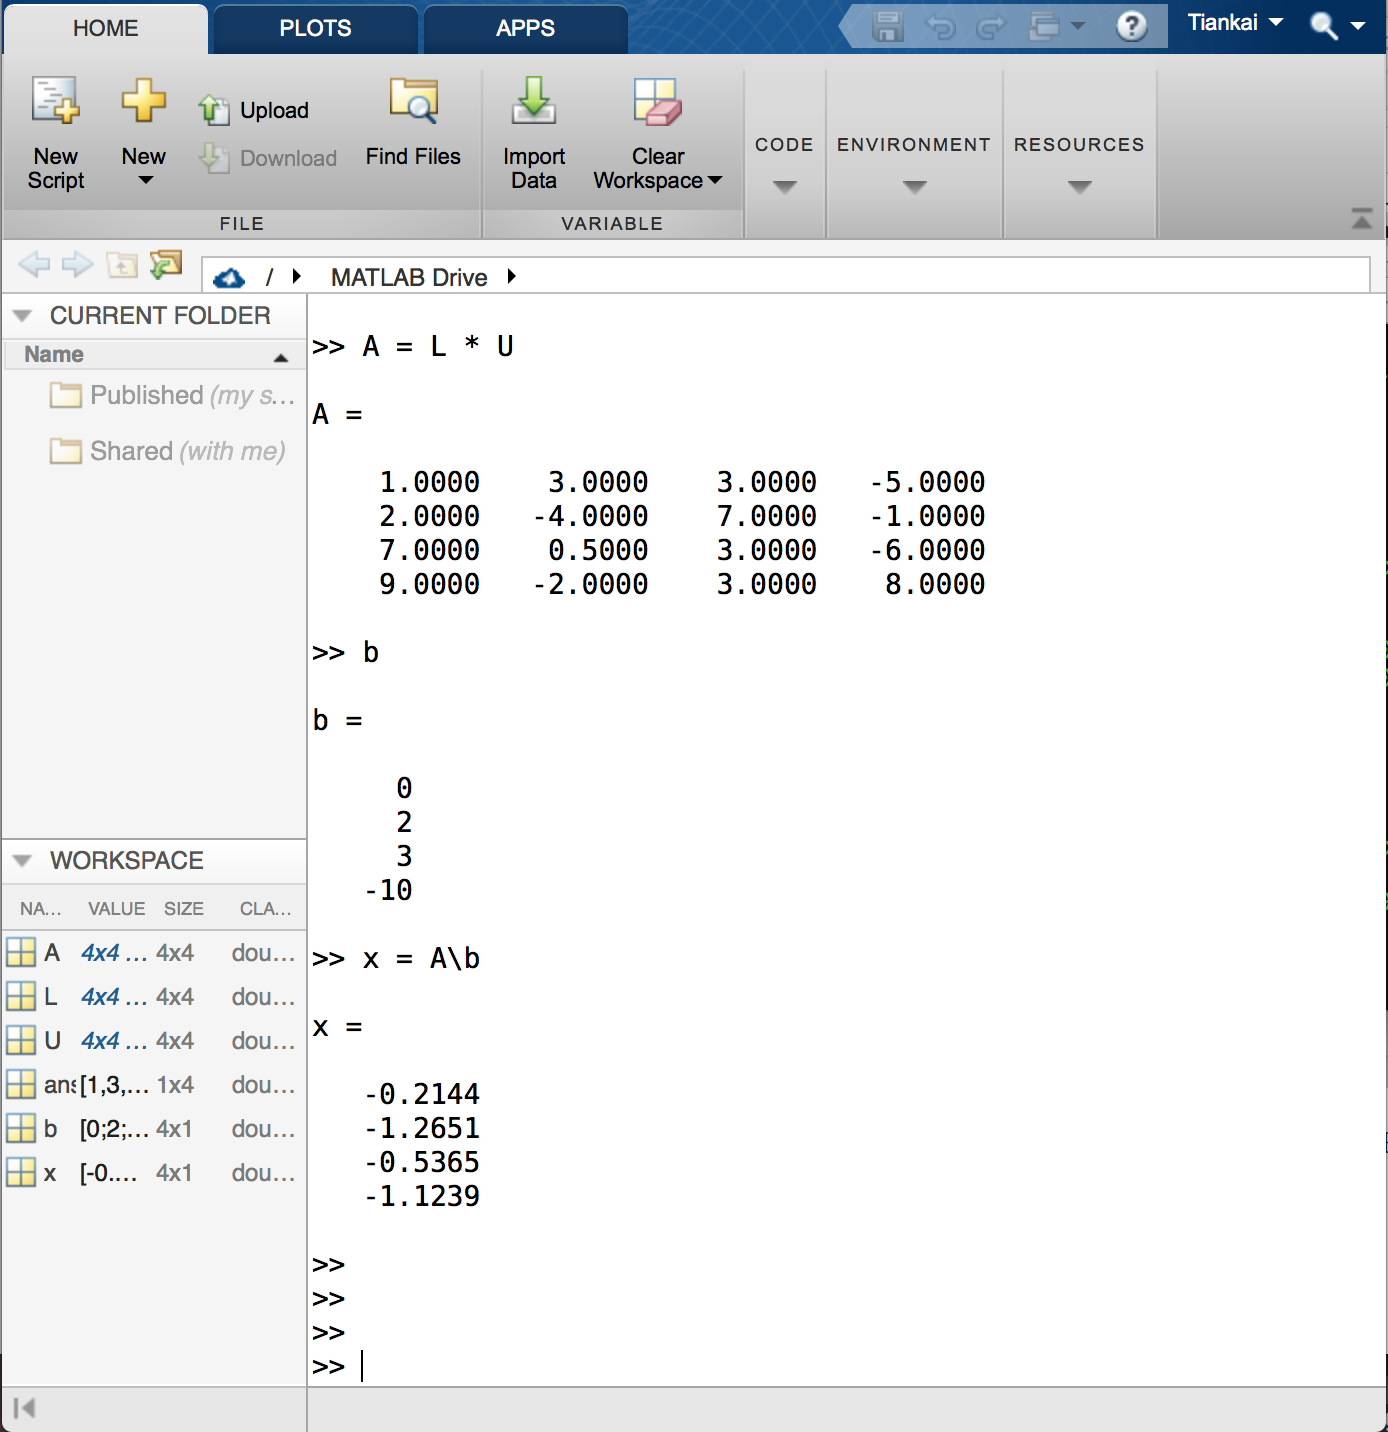
\includegraphics[width=0.6\textwidth]{matlab2.png}
  \caption{Verification of Ax = b in Matlab}
  \label{fig:matlab2}
\end{figure}


\section{Question 2}
\label{sec-2}

\subsection{Elaboration}
\label{sec-2-1}

\begin{itemize}
\item Calculating I and R

The problem is approached by setting the voltage at each node as a
variable to be determined. For any L, we have in total $(L + 1)^2$
nodes. For each node, we can use conservation of current to
generate a equation. By having the same number of equations as
unknowns, this linear system has a unique solution if the equations
are independent and the matrix is not singular.

The difficulty lies in the indexing of all the nodes i.e. to write
down the $(L+1)^2 \times (L+1)^2$ matrix. We choose to flatten the
$(L+1) \times (L+1)$ nodes with indices \texttt{i} and \texttt{j}. To elaborate,
instead of indexing the $(L+1)^2 \times (L+1)^2$ matrix by two
indices each runs from 0 to $(L+1)^2 - 1$, we use \texttt{i} and \texttt{j} each runs
from 0 to L. The equation associated with a node originally on the
grid at \texttt{i,j} will be the row with row number $(L+1) \times i + j$. The
column numbers are used to denote the contribution of current from
each neighboring nodes, which can be indexed by \texttt{i} $\to$ \texttt{i} $\pm$ \texttt{1} or
\texttt{j} $\to$ \texttt{j} $\pm$ \texttt{1}. In code, we need to treat the odd points at the
corners and sides differently. This is rather trivial and is easily
understood from reading the source code.

 Two nodes are special: A and B as indicated in the problem. As we
already know that V$_{\text{A}}$ = 0 and V$_{\text{B}}$ = 1, in the rows corresponding to
that node, we simply indicate only one contribution of current from
the node itself. In the result column vector b, we denote $b[0] = 0$
and $b[-1] = 1$ \footnote{Here we use the python notation b[-1] which means the last
element of the array b. In the actual c code, the index is directly keyed in.} such that the solution is V$_{\text{A}}$ = 0 and V$_{\text{B}}$
= 1. For all other entries of b, we put 0 as total current at each
intermediate node is zero.

Note that the contribution from each node must be multiplied by
$\sqrt{L}$ to take into account the resistance.

To calculate the total current, we only need the voltage from the
two neighboring nodes of A(or B) to calculate the two sources of
current and sum them up. The total resistance can be calculated by
$R = \frac{V}{I}$ accordingly.

\item Report calculation time

\texttt{time\_t} from \texttt{time.h} library is used to record two instances at the
start and the end of the programme. The difference is calculated and
converted to ms.
\end{itemize}


\subsection{Results}
\label{sec-2-2}

The results are presented in Table \ref{tbl:grid}. The processor
used is a 2.7GHz Intel Core i5. Since this programme is executed in
sequential, the number of cores does not matter. Answers for L = 1
and L = 2 are verified by hand.

\begin{longtable}{|c|c|c|c|}
\caption{\label{tbl:grid}Result from solving the grid with L.}
\\
\hline
L & Total current(units) & Total Resistance(units) & Time elapsed(ms)\\
\hline
\endhead
\hline\multicolumn{4}{r}{Continued on next page} \\
\endfoot
\endlastfoot
1 & 1.000000 & 1.000000 & <1\\
2 & 0.942809 & 1.060660 & <1\\
4 & 0.936170 & 1.068182 & <1\\
8 & 0.982735 & 1.017568 & 1\\
16 & 1.085307 & 0.921398 & 30\\
32 & 1.248904 & 0.800702 & 1289\\
64 & 1.483576 & 0.674047 & 74562\\
128 & aborted & aborted & aborted\\
\hline
\end{longtable}



For larger L such as L = 128, the matrix has $(128+1)^4 =
   276,922,881$ entries, each is a \texttt{double} that occupies 16 bytes. That
alone would take in total more than 4GB of the memory. Note that
the size of the problem grows by $\approx (L+1)^2$ instead of
L. Since LU decomposition is a $\textit{O}(n^a) \; (a>2)$ process, the
computing time escalates very fast for large L.

\pagebreak
\section{SRC}
\label{sec-3}

\begin{itemize}
\item \texttt{lab1\_1.c}
\end{itemize}
\hline
\begin{verbatim}
#include <stdio.h>
#include <stdlib.h>
#include "ludcmp.cpp"


int main(){

  int dim = 4;

  int *indx = (int *)malloc(dim * sizeof(int));
  float *d = malloc(sizeof(float));
  /* d needs to be a pointer to be refered to in det(A) */

  double **a = initMat(dim);

  a[0][0] = 1.0; a[0][1] = 3.0; a[0][2] = 3.0; a[0][3] = -5.0;
  a[1][0] = 2.0; a[1][1] = -4.0; a[1][2] = 7.0; a[1][3] = -1.0;
  a[2][0] = 7.0; a[2][1] = 1.0/2.0; a[2][2] = 3.0; a[2][3] = -6.0;
  a[3][0] = 9.0; a[3][1] = -2.0; a[3][2] = 3.0; a[3][3] = 8.0;

  printf("Matrix A recorded as:\n");
  printMat(a, dim);

  double *x = (double *)malloc(dim * sizeof(double));
  double *b = (double *)malloc(dim * sizeof(double));
  b[0] = 0.0; b[1] = 2.0; b[2] = 3.0; b[3] = -10.0;

  ludcmp(a, dim, indx, d, 1);

  printf("Matrix A after LU decomposition, stored in one single matrix:\n");
  printMat(a, dim);



  printf("For linear system Ax = b\n");
  printf("b = \n");
  printVec(b, dim);

  lubksb(a, b, x, dim, indx, 1);

  printf("Solving thought backward substitution, x = \n");
  printVec(x, dim);
}
\end{verbatim}

\hline

\pagebreak
\begin{itemize}
\item \texttt{lab1\_2.c}
\end{itemize}
\hline
\begin{verbatim}
#include <stdio.h>
#include <math.h>
#include <time.h>
#include "ludcmp.cpp"



int main(){

  time_t start, end;


  // Solve by setting the voltage of each node as a unknown. We have
  // L^2 unknowns and L^2 equations thus a unique solution can be
  // obtained. Notice that we already have V_00 = 0 and V_LL = 1
  int L;
  printf("Insert the dimension of the grid:\n");
  scanf("%d", &L);

  start = clock();              /* Start the timer */
  int dim = (L+1)*(L+1);        /* we have (L+1)^2 nodes in total */

  double **a = initMat(dim);

  for(int i = 0; i < dim; i++){
    for(int j = 0; j < dim; j++){
      a[i][j] = 0;              /* Since most values will be zero */
    }
  }

  double *x = (double *)malloc(dim * sizeof(double));
  double *b = (double *)malloc(dim * sizeof(double));
  for (int i = 0; i < dim; i++){b[i] = 0;} /* Summation of current is
                                              zero at each node */
  b[dim-1] = 1;                    /* This makes sure that V_LL = 1 */

  for(int i = 0; i<= L; i++){
    for(int j = 0; j<=L; j++){
      /* Assign equations for each node on the grid: */
      /* The row number (L * i + j) denote [i][j], the node we are
         concerning in this equation. The column number denotes the
         source of current from that node to node [i][j]*/
      if((i == 0 && j == 0) || (i == L && j == L)){
        /* This corresponds to point A or B where the voltage is 0 or
           1 hence do not need to be determined */
        a[(L+1) * i + j ][(L+1) * i + j] = 1; /* This will give us V_00 = 0
                                         and V_LL = 1*/

      }else if(i == 0 && j == L){ /* deal with the right bottom
                                       corner */
        /* Take L = 4 as an example */
        /* sqrt(L) [(V_03 - V_04) + (V_14 - V_04)] = 0 */
        a[(L+1) * i + j][(L+1) * i + j - 1]   = sqrt(L);
        a[(L+1) * i + j][(L+1) * (i + 1) + j] = sqrt(L);
        a[(L+1) * i + j][(L+1) * i + j]       = -2 * sqrt(L);

      }else if(i == L && j == 0){ /* Left top corner */
        a[(L+1) * i + j][(L+1) * (i - 1) + j] = sqrt(L);
        a[(L+1) * i + j][(L+1) * i + j +1]    = sqrt(L);
        a[(L+1) * i + j][(L+1) * i + j]       = -2 * sqrt(L);
      }else if(i == 0){
        a[(L+1) * i + j][(L+1) * (i + 1) + j] = sqrt(L);
        a[(L+1) * i + j][(L+1) * i + j + 1]   = sqrt(L);
        a[(L+1) * i + j][(L+1) * i + j - 1]   = sqrt(L);
        a[(L+1) * i + j][(L+1) * i + j]       = -3 * sqrt(L);
      }else if(i == L){
        a[(L+1) * i + j][(L+1) * (i - 1) + j] = sqrt(L);
        a[(L+1) * i + j][(L+1) * i + j + 1]   = sqrt(L);
        a[(L+1) * i + j][(L+1) * i + j - 1]   = sqrt(L);
        a[(L+1) * i + j][(L+1) * i + j]       = -3 * sqrt(L);
      }else if(j == 0){
        a[(L+1) * i + j][(L+1) * (i - 1) + j] = sqrt(L);
        a[(L+1) * i + j][(L+1) * (i + 1) + j] = sqrt(L);
        a[(L+1) * i + j][(L+1) * i + j + 1]   = sqrt(L);
        a[(L+1) * i + j][(L+1) * i + j]       = -3 * sqrt(L);
      }else if(j == L){
        a[(L+1) * i + j][(L+1) * (i - 1) + j] = sqrt(L);
        a[(L+1) * i + j][(L+1) * (i + 1) + j] = sqrt(L);
        a[(L+1) * i + j][(L+1) * i + j - 1]   = sqrt(L);
        a[(L+1) * i + j][(L+1) * i + j]       = -3 * sqrt(L);
      }else{
        a[(L+1) * i + j][(L+1) * (i - 1) + j] = sqrt(L);
        a[(L+1) * i + j][(L+1) * (i + 1) + j] = sqrt(L);
        a[(L+1) * i + j][(L+1) * i + j - 1]   = sqrt(L);
        a[(L+1) * i + j][(L+1) * i + j + 1]   = sqrt(L);
        a[(L+1) * i + j][(L+1) * i + j]       = -4 * sqrt(L);
      }
    }
  }

  int *indx = (int *)malloc(dim * sizeof(int));
  float *d = malloc(sizeof(float));

  ludcmp(a, dim, indx, d, 1);
  lubksb(a, b, x, dim, indx, 1);

  /* We need the two voltages next to point A to solve for the total
     current */

  double V_01, V_10;

  V_01 = x[1];
  V_10 = x[(L+1) * 1];

  double totalCurrent = sqrt(L)*(V_01 + V_10);
  double totalR = 1/totalCurrent;


  printf("Total current is %f\n", totalCurrent);
  printf("Total resistance is %f\n", totalR);

  end = clock();                /* End the timer */

  int t = (end-start) * 1000/CLOCKS_PER_SEC; /* Convert to ms */
  printf("Total running time to determine size of L = %d is %d ms\n", L, t);
}
\end{verbatim}

\hline

\pagebreak
\begin{itemize}
\item \texttt{ludcmp.cpp}
\end{itemize}
\hline
\begin{verbatim}
#include <stdio.h>
#include <math.h>
#include <stdlib.h>

double **initMat(int n){
  double **a = (double ** )malloc(n * sizeof(double *));
  for(int i = 0; i <n; i++)a[i] = (double *)malloc(n * sizeof(double));
  return a;
};

void printMat(double **a, int n){
  printf("\n");
  for(int i = 0; i < n ; i++){
    for(int j = 0; j < n ; j++){
      printf("  %f  ", a[i][j]);
    }
    printf("\n");
  }
};

void printVec(double *b, int n){
  printf("\n");
  for(int i = 0; i < n; i++){
    printf("  %f  ", b[i]);
  }
  printf("\n");
};

void ludcmp(double **a, int n, int *indx, float *d, int noPivot){

  const double TINY = 1.0e-40;

  int i, imax, j, k;
  double big, temp;
  double *vv;

  vv = (double *)malloc(n * sizeof(double));
  // d stores the information about row interchanges, for future
  // calculation of det(A)
  *d = 1.0;                     /* No row interchanges yet */


  for(i = 0; i<n; i++){        // loop over rows to get the implicit
    big = 0.0;                  // scalling information
    for(j = 0; j < n; j++)
      if((temp=fabs(a[i][j])) > big){ // fabs: returns absolute value
        big = temp;
      }
    if(big == 0.0) {
      printf("Singular matrix in routine ludcmp"); // throw error
    }
                                // No nonezero largest element.
    vv[i] = 1.0/big;            //save the scalling
  }
  for (k = 0; k< n; k++){       // This is the outermost k_ij loop
    big = 0.0;
    for (i = k; i < n; i++){
      temp = vv[i] * fabs(a[i][k]);
      if (temp > big){          // Is the figure of merit for the
        big = temp;             // pivot better than the best so far?
        imax = i;
      }
    }
    if (k != imax && !noPivot){
      for (j = 0; j < n; j++){
        temp = a[imax][j];
        a[imax][j] = a[k][j];
        a[k][j] = temp;
      }
      *d = -(*d);
      vv[imax] = vv[k];
    }
    indx[k] = imax;
    if (a[k][k] == 0.0){
      a[k][k] = TINY;
      // If the pivot element is zero, the matrix is singular
      // (at least to the precision of the algorithm).
      // For some applications on singular matricies, it is
      // desirable to substitute TINY to zero.
    }
    for (i = k +1; i < n; i++){
      temp = a[i][k] /= a[k][k]; // Divide by the pivot element
      for (j = k + 1; j < n; j++){ // Innermost loop: reduce remaining
                                // submatirx
        a[i][j] -= temp * a[k][j];
      }
    }
  }

  free(vv);

}

void lubksb(double **lu, double *b, double *x, int n, int *indx, int noPivot){

  int i, ii=0, ip, j;

  double sum;

  if(noPivot){
    for(int k = 0; k < n; k++){
      indx[k] = k;
    }
  }

  // make sure that the dimensions match

  for (i=0; i<n; i++) x[i] = b[i];
  for (i=0; i<n; i++){          // When ii is set to a positive value
      ip = indx[i];               // it will become the index of the first
      sum = x[ip];                // nonvanishing element of b. We now do
      x[ip] = x[i];               // the forward substitution.

    // The only new wrinkle is to unscramble the permutation as we go.
    if (ii != 0){
      for (j = ii-1; j<i; j++) sum -= lu[i][j]*x[j];
    }else if(sum != 0.0){       // A nonzero element was encountered,
      ii = i+1;                 // so from now on we will have to do the
    }                           // sums in the loop above
    x[i] = sum;
  }
  for (i = n-1; i>=0; i--){     // Now we do the bksb
    sum=x[i];
    for(j = i+1; j<n; j++) sum -= lu[i][j] * x[j];
    x[i] = sum/lu[i][i];        // Store a component of the solution vector X
  }

}
\end{verbatim}

\hline
% Emacs 25.2.1 (Org mode 8.2.10)
\end{document}
